% --------------------------------------------------------------
% This is all preamble stuff that you don't have to worry about.
% Head down to where it says "Start here"
% --------------------------------------------------------------

\documentclass[12pt]{article}

\usepackage[margin=1in]{geometry}
\usepackage{amsmath,amsthm,amssymb}
\usepackage{graphicx} %This allows to include eps figures
\usepackage{subcaption}
\usepackage[section]{placeins}
\usepackage{layout}
\usepackage{etoolbox}
\usepackage{mathabx}
\usepackage{courier}
% This is to include code
\usepackage{listings}
\usepackage{hyperref}
\usepackage{xcolor}
\definecolor{dkgreen}{rgb}{0,0.6,0}
\definecolor{gray}{rgb}{0.5,0.5,0.5}
\definecolor{mauve}{rgb}{0.58,0,0.82}
\lstdefinestyle{Python}{
    language        = Python,
    basicstyle      = \ttfamily,
    keywordstyle    = \color{blue},
    keywordstyle    = [2] \color{teal}, % just to check that it works
    stringstyle     = \color{green},
    commentstyle    = \color{red}\ttfamily
}

\newcommand{\N}{\mathbb{N}}
\newcommand{\R}{\mathbb{R}}
\newcommand{\X}{\mathbb{X}}
\newcommand{\Z}{\mathbb{Z}}
\def\doubleunderline#1{\underline{\underline{#1}}}

\newenvironment{theorem}[2][Theorem]{\begin{trivlist}
\item[\hskip \labelsep {\bfseries #1}\hskip \labelsep {\bfseries #2.}]}{\end{trivlist}}
\newenvironment{lemma}[2][Lemma]{\begin{trivlist}
\item[\hskip \labelsep {\bfseries #1}\hskip \labelsep {\bfseries #2.}]}{\end{trivlist}}
\newenvironment{exercise}[2][Exercise]{\begin{trivlist}
\item[\hskip \labelsep {\bfseries #1}\hskip \labelsep {\bfseries #2.}]}{\end{trivlist}}
\newenvironment{reflection}[2][Reflection]{\begin{trivlist}
\item[\hskip \labelsep {\bfseries #1}\hskip \labelsep {\bfseries #2.}]}{\end{trivlist}}
\newenvironment{proposition}[2][Proposition]{\begin{trivlist}
\item[\hskip \labelsep {\bfseries #1}\hskip \labelsep {\bfseries #2.}]}{\end{trivlist}}
\newenvironment{corollary}[2][Corollary]{\begin{trivlist}
\item[\hskip \labelsep {\bfseries #1}\hskip \labelsep {\bfseries #2.}]}{\end{trivlist}}

\begin{document}

% --------------------------------------------------------------
%                         Start here
% --------------------------------------------------------------

%\renewcommand{\qedsymbol}{\filledbox}

\title{Assignment 2 - Epipolar Geometry and 3D Reconstruction}%replace X with the appropriate number
\author{Nalet Meinen \\ %replace with your name
Computer Vision
}

\maketitle

\section{Part 1: The Eight Point Algorithm}

\subsection{Normalization Matrix}
The first part was to calculate the Normalization Matrix. This is described on the lecture notes as follows:
\begin{quote}
    Center the image data at the origin, and scale it so
    the mean squared distance between the origin and
    the data points is 2 pixels
\end{quote}

I began with calculating the centroid, then the mean squared distance. Important the mean of two norms results
in $\sqrt{2}$, that is why we devide $\frac{\sqrt{2}}{\mathrm{mean}}$.

\subsection{Eight Points Algorithm}

The formulas for the eight points algorithm where described in the slides from 23 - 35 (lecture 8). 
It is important to correctly calculate the matrix $A$, else the SVD is not possible. Slide 33 describes the algorithm
very well and is straight forward. For understanding purposes this 
\href{https://web.stanford.edu/class/cs231a/course_notes/03-epipolar-geometry.pdf}{PDF} from Standford
helped me to understand it better intuitively.

\begin{figure}[h!]
    \centering
    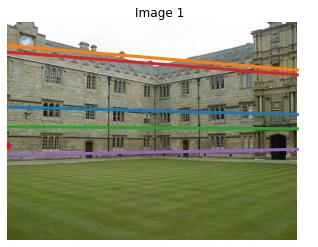
\includegraphics[scale=0.5]{eight_points.png}
    \caption{Result of the matched points}
\end{figure}

The results for the subsets of points were very accurate. In the first version of the 
code the plot of the line was slightly off where it should have been. This was corrected with
\texttt{x @ F}. The reason could be a transpose somewhere, which I did not find in the time given.

\subsection{Epipole and Epipolar Line}

\begin{figure}[h!]
    \centering
    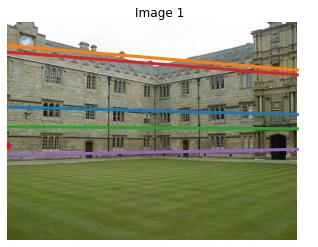
\includegraphics[scale=0.5]{eight_points.png}
    \caption{Epipolar line}
\end{figure}

Deriving a formula was easy. For that we convert the point itself to a line. With the multiplication with
$F$ we have then therefore the point/line in the new space. We know $x$. The MathLibPlot library can draw a line
between two points. So I calculated the y points at the border of the image and let the library draw the line.

The task where I must plot the point where the epipolar lines intersect is wrong. Obviously this point is
outside of the image as we would guess if I would have followed the lines. I guessed that if the task was written
this way the intersection point should be on the image.

\section{Part 2: 3D Model Reconstruction}

\subsection{Ransac}

Implementing the RANSAC algorithm took a lot of time. Here I first started an approach without the fundamental
matrix using only the distance, after merging the two points clouds in 2D.

\begin{figure}[h!]
    \centering
    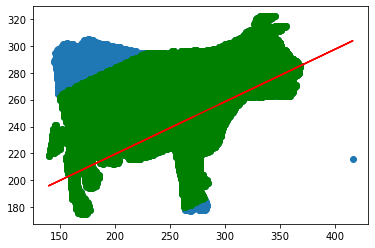
\includegraphics[scale=0.5]{ransac_inliners.png}
    \caption{RANSAC inliners}
\end{figure}

The dataset included two points that were intended as outliners. Finding a good line was difficult and then
fitting the line to the data, using then the inliers as the input for the eight-point algorithm.
Later I did discard this idea. The correct way was to use the eight-point algorithm as the model itself and then
use the least squared to calculate the distance to $F$.
The most difficult part here was to find the correct parameters to get RANSAC working correctly. I only managed 
to get rid of one outlier instead of the two in the data.

\subsection{Essential Matrix}
The calculation of the essential matrix was mentioned in the slides. The formula $E = I^T \cdot F \cdot I$ was
used.

\subsection{Decompose Essential Matrix}

For the decomposition of the essential matrix this 
\href{http://www.maths.lth.se/matematiklth/personal/calle/datorseende13/notes/forelas6.pdf}{PDF} from 
Lunds university helped me. Important are the matrices $W$ (rotation) and $Z$ (skew). In the first attempt
I tried to change the $W$ in order to get the result aligned to the coordinate-system (positive-wise). then
I saw that the provided image of the result is also "backward".

After enforcing rank two with $\mathrm{diag}([1,1,0])$ and rerunning the SVD. After, we get the two
rotations. Also, I got $S$ the two skew matrixes. As said before this 
\href{http://www.maths.lth.se/matematiklth/personal/calle/datorseende13/notes/forelas6.pdf}{PDF}
describes this very well on page 4.

\subsection{Reconstruction of the 3D Points}
\begin{figure}[h!]
    \centering
    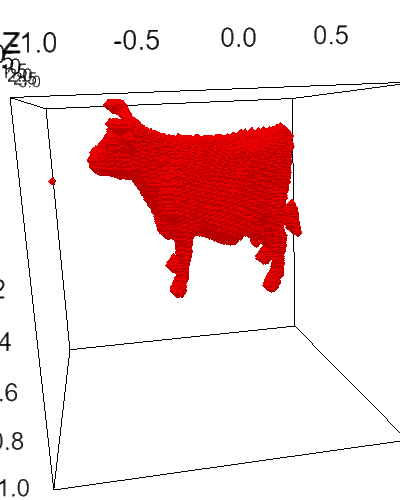
\includegraphics[scale=0.5]{3d_res.png}
    \caption{RANSAC inliners}
\end{figure}

As mentioned before, finding the different parameters for RANSAC was difficult and time-consuming. 
The decomposition is not unique. Depending on how I ran RANSAC, I had to change $E$ to $-E$ and 
vice-versa. A good thing was that this issue was also mentioned on the piazza website. This result was one of 
the better ones. Unfortunately, I did not found a way to make also the second outliner disappear.

In part (b) I had to calculate the error of the model. I was provided with homogenous coordinates which 
had to be converted. $H_{\mathrm{ground truth}} = H r_{\mathrm{ground truth}} H l_{\mathrm{ground truth}}^{-1}$.

As written in the task, I converted the matrix in Euler angles. With the obtained data we then got the results:

\begin{itemize}
    \item error on angles: 51.5°
    \item error on translation: 1.1
  \end{itemize}
\end{document}